\documentclass[11pt,a4paper]{article}
\usepackage[margin=25mm]{geometry}
\usepackage[T1]{fontenc}
\usepackage{mathpazo,amsmath,amssymb,graphicx,booktabs,longtable,array,caption,setspace,microtype}
\usepackage[hidelinks]{hyperref}
\usepackage{fancyhdr}
\setstretch{1.15}
\setlength{\parskip}{4pt}
\setlength{\parindent}{0pt}
\captionsetup{font=small,labelfont=bf}
\pagestyle{fancy}\fancyhf{}\fancyhead[L]{\small GBD 2023: cause-specific infertility}\fancyhead[R]{\small Research draft}\fancyfoot[C]{\thepage}
\setlength{\headheight}{14pt}
\setlength{\emergencystretch}{2em}
\newcommand{\ASPR}{\mathrm{ASPR}}
\title{Age-specific contrasts and demographic contributions to PCOS- and endometriosis-related infertility in China and the other G20 countries, 1990--2023}
\author{Research manuscript draft\\\small Author names, affiliations and correspondence to be supplied by the research team}
\date{25 October 2026}
\begin{document}
\maketitle
\begin{center}\small Secondary descriptive analysis of the Global Burden of Disease Study 2023\end{center}
\begin{abstract}
\noindent\textbf{Background:} Population and infertility-type composition can obscure international contrasts in cause-specific infertility. We compared China with an age-specific population-pooled reference comprising the other 18 sovereign G20 countries.

\noindent\textbf{Methods:} We analyzed GBD 2023 female infertility attributed to polycystic ovarian syndrome (PCOS) and endometriosis at ages 15--49, 1990--2023. We estimated restricted-age standardized prevalence, rate differences and ratios, age and infertility-type contributions, and Shapley decompositions of case-count changes. Sensitivities examined country composition, age range, trends and endpoints. Derived quantities were point estimates because jointly aligned uncertainty draws were unavailable.

\noindent\textbf{Results:} China's total PCOS-related infertility standardized prevalence increased from 333.56 to 605.08 per 100,000, versus 606.48 to 726.45 in the reference. The rate ratio rose from 0.550 to 0.833. In 2023, the primary-infertility difference was $-123.54$, whereas the secondary-infertility difference was +2.16. Secondary infertility accounted for 69.4\% of the change in the total difference. China's PCOS-related modeled count increased by 783,425; changing age-specific prevalence contributed +860,721, with demographic offsets. For endometriosis-related infertility, opposing primary ($-7.94$) and secondary (+7.73) differences nearly canceled in 2023. The total difference was $-0.20$ in 2023 but $-8.76$ in 2022, demonstrating endpoint sensitivity. No evaluated forecasting model consistently outperformed the naive baseline across all ages and validation schemes.

\noindent\textbf{Conclusions:} Aggregate contrasts concealed distinct primary and secondary infertility patterns. Rising modeled PCOS-related age-specific prevalence outweighed demographic offsets in China, while endometriosis comparisons depended strongly on the terminal year. These descriptive estimates require uncertainty-qualified and independent epidemiological corroboration.
\end{abstract}
\textbf{Keywords:} infertility; polycystic ovarian syndrome; endometriosis; GBD 2023; age standardization; demographic decomposition; China; G20

\section{Introduction}
Endometriosis and polycystic ovarian syndrome (PCOS) have distinct clinical manifestations and implications for reproductive health. Contemporary clinical guidance addresses fertility within broader, individualized management of both conditions \cite{pcos,eshre}. Population estimates of infertility attributed to these conditions answer a narrower question than estimates of their total disease prevalence or disability. Conflating these outcomes can substantially distort the interpretation of trends and international comparisons.

GBD provides comparable modeled estimates across locations and years, including infertility attributed to specific underlying causes \cite{gbd}. Existing analyses have already described the global, regional and national burden of endometriosis, PCOS and unexplained infertility, including their attribution to infertility \cite{xu}. A recent study also examined and projected endometriosis- and PCOS-related infertility among women aged 15--49 years in China and globally using GBD 2021 \cite{lu}. Consequently, a change in database edition or an expanded set of comparison countries is insufficient by itself to establish a new scientific contribution.

A useful complementary question concerns the construction and interpretation of international contrasts. A group average of country-level standardized rates does not generally reproduce the rate obtained by pooling age-specific numerators and denominators. The composition of a reference group can also change over time. Moreover, aggregate convergence can conceal opposing age-specific contributions, while changes in case counts can result from changes in reproductive-age population size, the distribution of ages within that population, or age-specific prevalence.

We therefore examined China relative to the other 18 sovereign G20 countries using an explicitly population-pooled reference. The objectives were to describe the magnitude, age pattern and primary/secondary infertility composition of these contrasts, identify the arithmetic contributions to changes in China's case counts, and evaluate robustness to reference construction and analytic choices. An additional analysis assessed endpoint sensitivity after inspection revealed a marked terminal-year change in the endometriosis series. We treated these as analyses of modeled population estimates, rather than direct observations of individual infertility or causal evaluations of policy.

\section{Methods}
\subsection{Design, sources and population}
This ecological secondary analysis used GBD 2023 Results Tool downloads obtained on 25 October 2026 \cite{results}. The analysis covered 1990--2023, females aged 15--49 years, and seven five-year age groups. Countries were China, Argentina, Australia, Brazil, Canada, France, Germany, India, Indonesia, Italy, Japan, Republic of Korea, Mexico, Russian Federation, Saudi Arabia, South Africa, T\"urkiye, United Kingdom, and United States of America. This fixed set represents the 19 sovereign country members of the G20; regional organizations were not treated as countries. The reference excluded China throughout.

We selected the infertility impairment (identifier 198), with underlying causes endometriosis (607) and PCOS (605), prevalence and years lived with disability (YLDs), and Number and Rate metrics. Female population estimates were downloaded from the same GBD release for matching locations, years and ages. The primary endpoint combined primary and secondary infertility as total infertility. Supplementary exports separately identified primary infertility (220) and secondary infertility (221). Annual stratum-specific Number estimates were divided by matching population to reconstruct rates; original Number and Rate exports for 1990 and 2023 independently checked this reconstruction. This reduced redundant exported metrics after a combined annual request exceeded the remaining account download allowance. No individual-level records were accessed.

The GBD methods appendix describes survey-based primary infertility in couples without a previous live birth who desire a child, have been in a union for at least five years, and report no contraceptive use. Secondary infertility additionally uses the interval since the last live birth. These survey definitions and clinical source definitions are harmonized within the GBD modeling framework; they should not be equated directly with a uniform 12-month clinical definition. Cause-specific infertility is allocated within the modeled envelope; it is not simply the prevalence of the underlying disease \cite{gbd}.

\subsection{Quality assurance and standardization}
Before analysis, we required complete coverage of all combinations of location, year, age, cause, measure and metric, unique dimensional keys, consistent identifiers, non-negative finite values and ordered original lower limits, point estimates and upper limits. We independently compared Number divided by matching female population with the official Rate, using the rate scale of 100,000. Original files, acquisition identifiers and SHA-256 hashes were retained. An independent pilot export for China, age 35--39 in 2023, provided an additional extraction check.

We used the GBD 2023 standard age weights reproduced to six decimal places in a published supplementary table \cite{chen}, normalized within ages 15--49. This published reproduction was available; the original machine-precision IHME weight file was not retrieved. The unnormalized weights were 0.082891, 0.078012, 0.075914, 0.073217, 0.068281, 0.061474 and 0.055113, respectively. All standardized rates reported here are restricted-age rates and are not all-age GBD standardized rates.

For age $a$, country $c$, year $t$, case count $C_{cat}$ and female population $P_{cat}$, let $r_{cat}=10^5 C_{cat}/P_{cat}$. With normalized standard weights $w_a$, we calculated
\begin{equation}
 \ASPR_{ct}=\sum_a w_a r_{cat},\qquad
 r_{Rt,a}=10^5\frac{\sum_{c\ne\mathrm{China}}C_{cat}}{\sum_{c\ne\mathrm{China}}P_{cat}}.
\end{equation}
The reference rate was standardized after pooling within ages. YLD rates were calculated in the same manner using YLD numerators. Absolute counts were summed without standardization. We did not average national standardized rates to construct the main reference.

\subsection{Contrasts and age contributions}
Writing $C$ for China, the absolute contrast was $D_t=\ASPR_{C,t}-\ASPR_{R,t}$; the relative contrast was $RR_t=\ASPR_{C,t}/\ASPR_{R,t}$. Negative $D_t$ indicates a lower modeled rate in China. Changes in the contrast were decomposed exactly by age:
\begin{equation}
 D_T-D_0=\sum_a w_a\left[(r_{\mathrm{China},aT}-r_{R,aT})-(r_{\mathrm{China},a0}-r_{R,a0})\right].
\end{equation}
A positive contribution indicates movement of the signed difference toward more positive values; it need not represent a beneficial change. We also calculated a same-population benchmark,
\begin{equation}
 B_T=\sum_a P_{\mathrm{China},aT}(r_{\mathrm{China},aT}-r_{R,aT})/10^5.
\end{equation}
This signed arithmetic contrast applies reference age-specific rates to China's actual population. It is not an estimate of preventable cases, a treatment effect, or an attainable policy target.

\subsection{Decomposition of case-count changes}
We expressed the case count as $F(N,\boldsymbol f,\boldsymbol p)=N\sum_a f_a p_a$, where $N$ is the total female population aged 15--49, $f_a$ is its age distribution, and $p_a$ is age-specific prevalence as a proportion. For each factor, we averaged its marginal contribution across all six possible replacement orders between the starting and ending states. These Shapley contributions sum exactly to the observed modeled case-count change. We examined 1990--2023 and 2010--2023 for both causes in all 19 countries. Population size here refers specifically to females aged 15--49; age composition refers to redistribution within this range. The age-specific prevalence component includes epidemiological change, ascertainment and modeling changes and cannot be interpreted as a causal risk-factor contribution.

\subsection{Trends, sensitivities and forecast validation}
We fitted continuous piecewise linear models to log standardized rates, searching integer-year knot locations with zero to two knots and at least five observations per segment, counting shared boundary years in each segment. Model selection used the Bayesian information criterion, including a penalty for knot locations. Segment-specific annual percentage change was $100[\exp(\beta)-1]$; average annual percentage change (AAPC) was obtained from duration-weighted log slopes. These fits summarize modeled trajectories and are not outputs of the proprietary Joinpoint program. AR(1) generalized least-squares refits retained the OLS-selected knots; allowing up to three knots and restricting the period to 2010--2023 were additional sensitivities. Trend confidence intervals are conditional on selected knots and fixed GBD point estimates.

Reference sensitivities used age-specific country population shares fixed at 1990, excluded one reference country at a time, and restricted ages to 20--49 with renormalized weights. Following inspection of the terminal-year endometriosis increase, we added analyses ending in 2021 and 2022; these endpoint analyses were not prespecified. To evaluate numerical sensitivity to published weight rounding, we evaluated all $2^7$ combinations of perturbing unnormalized weights by $\pm0.5\times10^{-6}$. The resulting deterministic envelopes are not uncertainty intervals.

An exploratory forecasting module evaluated each Chinese age-specific prevalence series on the logit scale. Candidates were a constant-last-rate baseline, ARIMA with $p,q\in\{0,1,2\}$ and $d\in\{0,1\}$ selected by training-set corrected AIC, and additive damped-trend exponential smoothing. ARIMA candidates failing convergence were excluded. Rolling training windows contained at least 20 years and assessed horizons 1, 3 and 5; a separate last-10-year holdout assessed horizons 1--10. We specified an exploratory retention rule before running this module: at least 10\% lower mean absolute error (MAE) than the baseline in every age group in both validation schemes, with complete predictions. Future counts would additionally require compatible population projections; none were generated when validation failed. This module was not a validation against independent observed infertility data.

\subsection{Uncertainty, reproducibility and reporting}
Downloaded files contained original marginal uncertainty limits but no jointly aligned draws across ages, locations and years. We preserved original limits but did not sum their endpoints, treat them as standard errors, or construct derived uncertainty intervals for pooled rates, contrasts, contributions or decompositions. Accordingly, cross-country contrasts are descriptive point estimates and no significance claims are made. Conditional trend intervals exclude GBD uncertainty, knot-selection uncertainty and structural model uncertainty. Python 3.12, NumPy, pandas, SciPy, statsmodels and Matplotlib were used; pinned dependencies, analysis code and derived outputs are provided at \url{https://github.com/jiabao1314/PCOS}. Applicable GATHER reporting items are mapped in the Supplement \cite{gather}.

\section{Results}
\subsection{Data completeness and overall contrasts}
The burden export contained 36,176 rows, exactly matching 19 countries, 34 years, seven ages, two causes, two measures and two metrics. The population export contained 4,522 matching age--country--year cells. An additional 36,176 annual Number rows covered both infertility types, measures and causes; 4,256 endpoint Number/Rate rows independently validated them. Primary plus secondary point estimates reproduced total infertility throughout the grid. There were no duplicate analytical cells or unordered original bounds. Reconstructed rates agreed with official rates to a maximum absolute discrepancy of $1.51\times10^{-11}$ per 100,000, supporting denominator and unit consistency.

For PCOS-related infertility, China's ASPR increased from 333.56 in 1990 to 605.08 per 100,000 in 2023, compared with 606.48 to 726.45 in the reference (Table~\ref{tab:prevalence}). The difference changed from $-272.92$ to $-121.38$ and the ratio from 0.550 to 0.833. China's modeled prevalent cases increased from approximately 1.083 to 1.867 million, whereas reference cases increased from 3.446 to 6.124 million. The direction of the China/reference contrast remained negative across all years (Figure~\ref{fig:trends}). Country-specific rates showed substantial heterogeneity (Figure~\ref{fig:countries}); these rankings are descriptive because joint uncertainty was unavailable.

For endometriosis-related infertility, China's ASPR was 63.70 in 1990 and 53.30 in 2023, versus 66.63 and 53.51 in the reference. The corresponding difference changed from $-2.93$ to $-0.20$ per 100,000, with a 2023 ratio of 0.996. China's modeled count decreased from 192,845 to 181,587. However, this endpoint comparison concealed important non-monotonicity, including a marked increase from 43.13 in 2022 to 53.30 in 2023, approximately 23.6\%. The difference in 2022 was $-8.76$, and its change since 1990 was $-5.83$, compared with +2.73 when ending in 2023 (Table~\ref{tab:endpoint}). Thus, even the direction of the long-period change in this signed difference depended on the final year.

\begin{table}[htbp]\centering\small
\caption{Restricted-age standardized prevalence and modeled case counts, ages 15--49.}\label{tab:prevalence}
\setlength{\tabcolsep}{3.5pt}
\begin{tabular}{llrrrrrr}\toprule
 & & \multicolumn{2}{c}{Cases, thousands} & \multicolumn{2}{c}{ASPR per 100,000} & & \\
Cause & Year & China & Reference & China & Reference & $D$ & $RR$\\\midrule
Endometriosis & 1990 & 192.8 & 375.6 & 63.70 & 66.63 & -2.93 & 0.956 \\
Endometriosis & 2023 & 181.6 & 457.1 & 53.30 & 53.51 & -0.20 & 0.996 \\
PCOS & 1990 & 1,083.3 & 3,446.2 & 333.56 & 606.48 & -272.92 & 0.550 \\
PCOS & 2023 & 1,866.7 & 6,124.2 & 605.08 & 726.45 & -121.38 & 0.833 \\
\bottomrule
\end{tabular}
\caption*{Reference: age-specific population-pooled rates for the other 18 sovereign G20 countries. All cells are point estimates. $D$: China minus reference; $RR$: China/reference. PCOS: polycystic ovarian syndrome.}
\end{table}

\subsection{Contrasting primary and secondary infertility}
The total PCOS contrast combined a marked primary-infertility difference with near parity in secondary infertility (Table~\ref{tab:strata}; Figure~\ref{fig:strata}). In 2023, primary-infertility ASPRs were 97.35 in China and 220.89 in the reference ($D=-123.54$, $RR=0.441$); secondary-infertility ASPRs were 507.72 and 505.56 ($D=+2.16$, $RR=1.004$). Between 1990 and 2023, the primary difference changed by +46.40 and the secondary difference by +105.14 per 100,000, together reproducing the +151.54 total change. Secondary infertility therefore accounted for 69.4\% of that signed change. Its 2023 difference ranged from $-113.63$ to +30.72 in leave-one-country-out comparisons, so the small positive main contrast was not robust to reference composition. Primary infertility remained lower in China in every country-exclusion analysis.

For endometriosis, the 2023 primary difference was $-7.94$ and the secondary difference +7.73, nearly canceling in the total contrast. The primary and secondary signs persisted across country-exclusion references in 2023, but the secondary endpoint change remained important: its difference was $-0.40$ in 2022. Thus, cancellation by infertility type and sensitivity to the terminal year both shaped the aggregate result. These decompositions concern modeled infertility categories and do not establish individual transitions between primary and secondary infertility.

\subsection{Age pattern and same-population benchmarks}
For PCOS, ages 40--44 and 35--39 contributed +33.60 and +31.07 per 100,000, respectively, to the +151.54 change in $D$ between 1990 and 2023. Together they accounted for approximately 42.7\% of the signed net change. Contributions from ages 20--34 and 45--49 were also positive; ages 15--19 contributed $-1.46$. These are contributions to a standardized contrast, rather than counts or causal effects (Figure~\ref{fig:ages}).

Endometriosis showed a different age pattern. Ages 20--44 made positive contributions to the 1990--2023 change in $D$, partly offset by ages 15--19 and 45--49. A positive age-specific contrast persisted at older reproductive ages even while several younger groups had negative contrasts. The 2023 same-Chinese-population benchmark was +6,721 cases for endometriosis-related infertility and $-390,747$ for PCOS-related infertility (Figure~\ref{fig:decomp}). The positive endometriosis count benchmark alongside a slightly negative standardized difference reflects different weighting: China's actual age distribution for the count benchmark and a common standard distribution for the rate difference.

\subsection{Contributions to case-count changes}
Between 1990 and 2023, China's PCOS-related infertility count increased by 783,425. Changing age-specific prevalence contributed +860,721 cases, while changes in reproductive-age female population size and age composition contributed $-68,426$ and $-8,869$, respectively (Table~\ref{tab:decomp}). Therefore, the prevalence component exceeded the net increase because demographic components offset part of it. The same direction of components was observed when ending in 2021 or 2022 (Supplementary machine-readable endpoint decomposition).

For endometriosis-related infertility, the net change was $-11,258$ cases. Population size contributed $-8,660$, age composition +30,818, and age-specific prevalence $-33,417$. The terminal-year choice changed the magnitudes substantially: the 1990--2022 net change was $-43,653$, with an age-specific prevalence contribution of $-67,157$. These decompositions are exact accounting identities based on modeled prevalence and population; they do not establish why age-specific prevalence changed.

\begin{table}[htbp]\centering\small
\caption{Shapley decomposition of changes in China's modeled prevalent cases, thousands.}\label{tab:decomp}
\setlength{\tabcolsep}{4pt}
\begin{tabular}{llrrrr}\toprule
Cause & Period & Net change & Population size & Age composition & Prevalence\\\midrule
Endometriosis & 1990--2023 & -11.3 & -8.7 & 30.8 & -33.4 \\
Endometriosis & 2010--2023 & 6.1 & -38.4 & 7.7 & 36.8 \\
PCOS & 1990--2023 & 783.4 & -68.4 & -8.9 & 860.7 \\
PCOS & 2010--2023 & -129.8 & -414.4 & -18.2 & 302.9 \\
\bottomrule
\end{tabular}
\caption*{Population size is the female population aged 15--49; age composition is its within-range distribution; prevalence is age-specific modeled infertility prevalence. Contributions may exceed the net change and need not have the same sign. Rounding can cause small displayed discrepancies.}
\end{table}

\subsection{Trends and robustness}
For 1990--2023, OLS segmented-model AAPCs for PCOS-related infertility were +1.89\% in China and +0.53\% in the reference. AR(1) refits gave +1.94\% and +0.49\%, respectively. Endometriosis AAPCs were $-0.86$\% and $-0.74$\% under OLS and $-0.82$\% and $-0.74$\% under AR(1). These summaries were conditional on the model and did not imply statistically established differences between countries or causes (Table~\ref{tab:trends}).

In 2023, PCOS differences remained negative across all leave-one-country-out references, ranging from $-315.15$ when excluding India to $-82.67$ when excluding the United States. Fixing age-specific country shares at 1990 yielded $D=-202.48$; restricting to ages 20--49 yielded $D=-149.85$. Thus, the direction was stable but the magnitude depended materially on the reference. For endometriosis, leave-one-out differences ranged from $-2.61$ to +1.81; the 20--49 contrast was +0.15 (Figure~\ref{fig:sensitivity}). Statements that China was definitively above or below the reference would therefore be unwarranted. Published-weight rounding did not reverse the main 2023 contrast signs within the evaluated numerical envelopes.

The YLD comparisons had the same broad direction as prevalence: China's standardized YLD rate increased for PCOS and declined for endometriosis between 1990 and 2023, remaining below the reference at the terminal year (Table~\ref{tab:yld}; Figure~\ref{fig:yld}). These outcomes share the GBD modeling framework and should not be interpreted as independent replications.

\subsection{Forecast validation}
Neither ARIMA nor damped exponential smoothing met the retention criterion for either cause. Across ages and validation schemes, the worst MAE ratios relative to the naive baseline were 1.80 and 2.10 for endometriosis and 2.20 and 1.79 for PCOS, respectively (Table~\ref{tab:forecast}). Accordingly, long-range rate trajectories and future case counts were not presented. The validation tables retain all age-specific predictions and errors, including the terminal-year deviations.

\section{Discussion}
This analysis identifies two distinct patterns in China's modeled cause-specific infertility burden. First, the PCOS-related infertility rate increased faster than that of the population-pooled comparison, narrowing a negative rate difference while remaining below the reference under every country-exclusion sensitivity. Second, the endometriosis contrast was much smaller in 2023 but highly dependent on endpoint choice. Presenting only starting and ending values would have obscured that the endometriosis difference had become more negative through 2022 before the terminal-year change.

The infertility-type analysis further changes the interpretation of the aggregate PCOS difference. A persistent primary-infertility deficit coexisted with secondary-infertility rates close to the reference by 2023. Most of the narrowing in the total standardized difference corresponded arithmetically to the secondary category. For endometriosis, near parity in the total rate concealed opposing subtype contrasts. These are distinct estimands: a low total contrast does not imply that either subtype has a low contrast, and a secondary-infertility increase cannot be interpreted as an observed transition in individual women.

The PCOS decomposition separates increased modeled age-specific prevalence from demographic change. The decrease in the total number of women aged 15--49 and the change in its internal age composition offset rather than explained the net case increase. This matters for interpretation: a rising case count does not automatically mean that population growth is the principal contributor, and overall national aging is not equivalent to aging within the reproductive-age denominator. The large contributions from ages 35--44 to the changing standardized contrast further indicate that an all-ages summary alone misses relevant heterogeneity. These descriptive findings can inform surveillance priorities, but do not establish mechanisms such as changes in obesity, reproductive timing, diagnosis, treatment access, or fertility intentions.

Our analyses complement previous GBD studies of the same infertility causes \cite{xu,lu} by making reference construction explicit and linking age-specific contrasts to case-count accounting. Pooling numerators and denominators within age groups yields a reference interpretable as the aggregate rate in the comparison population. Nevertheless, it gives substantial influence to populous countries. The difference between current population pooling and fixed 1990 country shares shows that changes in reference composition affect the magnitude of convergence. The large influence of India on the PCOS contrast demonstrates why the reference should not be interpreted as a neutral standard of ideal reproductive health.

The endometriosis endpoint result requires particular caution. The 2023 jump was present in the downloaded official estimates and was consistent with an independently obtained pilot cell. Internal consistency of data extraction does not validate the underlying epidemiological change. Shared changes in source inputs, disease models, cause attribution, or exposure patterns could affect multiple outputs together. We cannot determine the explanation from the aggregate files. The persistence of a substantially negative difference through 2022, followed by near parity in 2023, argues for independent corroboration before treating the terminal-year result as a sustained shift. The endpoint sensitivity was prompted by inspection and should be recognized as such.

The same-population benchmark adds another interpretive safeguard. Its sign can differ from the standardized rate contrast because it uses China's actual age distribution. For endometriosis, the older-age positive differences had sufficient weight to produce a positive count benchmark despite a slightly negative standardized difference. This is a consequence of the estimands, not a contradiction. Neither benchmark quantifies preventable cases: the comparison populations differ in exposures, fertility histories, diagnosis and care, and the modeled contrasts do not isolate a modifiable causal pathway.

Clinical guidance for PCOS emphasizes reproductive, metabolic and psychological assessment across the life course; endometriosis guidance also situates fertility decisions within broader individualized care \cite{pcos,eshre}. Our findings support the need for age-specific population monitoring alongside such care, but they cannot select a treatment or estimate its impact. Lower modeled prevalence should not be interpreted automatically as better access to diagnosis or treatment, and convergence toward a reference with increasing rates is not necessarily progress.

Forecast evaluation provided a further limit on interpretation. More complex models did not reliably improve on the simple baseline across ages and validation schemes. Suppressing unsupported long-range forecasts therefore reflects the planned conditional approach rather than a claim that future burden will remain constant. Backtesting the GBD series itself also cannot establish predictive validity for subsequently observed infertility. Reliable future count scenarios would require a clearly specified population projection, assumptions about age-specific rates, and explicit separation of demographic and epidemiological uncertainty.

Several limitations affect this analysis. GBD estimates integrate heterogeneous and sometimes sparse underlying evidence; cross-country comparability remains conditional on its modeling assumptions \cite{gbd}. The etiologic attribution and modeled infertility envelope do not identify infertility among every clinically diagnosed patient with PCOS or endometriosis. Our population denominator includes all women in the specified ages, rather than only couples currently attempting pregnancy. Aggregate ecological estimates cannot identify individual risks or policy effects.

The absence of aligned draws is especially important: all pooled, standardized and decomposed results lack propagated GBD uncertainty. Marginal lower and upper limits cannot be combined as though they were joint draws. Conditional trend intervals are narrower in scope than epidemiological uncertainty and should not be used to infer established international differences. In addition, the standard weights came from a rounded published reproduction; numerical perturbation assessed rounding but could not verify the original machine-precision file or remove upstream source uncertainty. Annual stratum rates were reconstructed from original Number estimates and matching population, with agreement verified against independent official endpoint rates. This arithmetic consistency does not remove uncertainty in the underlying infertility attribution. The fixed G20 country set is economically defined and is neither a matched causal comparison nor representative of all global regions. Finally, endpoint sensitivity and the explicit forecasting retention rule were added during execution and were not externally preregistered.

\section{Conclusions}
Within GBD 2023 modeled estimates, China's increase in PCOS-related infertility cases reflected rising age-specific prevalence that outweighed demographic offsets. The negative total contrast with the other 18 sovereign G20 countries narrowed but persisted across reference sensitivities; a large primary-infertility deficit coexisted with secondary-infertility rates close to the reference. For endometriosis-related infertility, apparent near parity in 2023 was not a stable summary of the preceding trajectory. Transparent age-specific pooling, decomposition and sensitivity analyses are necessary to distinguish these patterns; causal and uncertainty-qualified conclusions require additional evidence.

\section*{Declarations}
\textbf{Ethics and consent:} This secondary analysis used aggregated GBD outputs without individual participant records. The responsible authors must verify the applicable local ethics determination before submission; no new institutional approval or waiver is claimed here.

\textbf{Data and code availability:} Data were obtained from the GBD Results Tool, subject to IHME's applicable terms. Exact query identifiers, country mapping, input hashes, normalization code and derived outputs accompany the repository. Original downloads are retained in the research workspace and the user's designated Drive archive; public repository distribution focuses on code and derived results. Original marginal uncertainty limits are preserved in the downloads.

\textbf{Authorship, funding and competing interests:} To be completed and verified by the research team. No author contribution, funding status or absence of competing interests has been assumed.

\textbf{Assistance disclosure:} AI-assisted coding, analysis orchestration and manuscript drafting were used in preparing this draft. Human authors remain responsible for source verification, analysis review, interpretation and the journal-specific disclosure.

{\small\setstretch{1.0}
\begin{thebibliography}{9}
\bibitem{pcos} Teede HJ, Tay CT, Laven JJE, et al. Recommendations from the 2023 International Evidence-based Guideline for the Assessment and Management of Polycystic Ovary Syndrome. \emph{J Clin Endocrinol Metab}. 2023;108:2447--2469. \href{https://doi.org/10.1210/clinem/dgad463}{doi:10.1210/clinem/dgad463}.
\bibitem{eshre} Becker CM, Bokor A, Heikinheimo O, et al. ESHRE guideline: endometriosis. \emph{Hum Reprod Open}. 2022;2022:hoac009. \href{https://doi.org/10.1093/hropen/hoac009}{doi:10.1093/hropen/hoac009}.
\bibitem{gbd} GBD 2023 Collaborators. Burden of 375 diseases and injuries, risk-attributable burden of 88 risk factors, and healthy life expectancy in 204 countries and territories, including 660 subnational locations, 1990--2023: a systematic analysis for the Global Burden of Disease Study 2023. \emph{Lancet}. 2025. \href{https://doi.org/10.1016/S0140-6736(25)01637-X}{doi:10.1016/S0140-6736(25)01637-X}. Includes Supplementary Appendix 1, infertility methods.
\bibitem{xu} Xu Y, Jia Y, Li Q, et al. Global, regional, and national burden of endometriosis, PCOS, and unexplained infertility and their attribution to infertility, 1990--2021: Global Burden of Disease Study 2021. \emph{J Evid Based Med}. 2025;18:e70100. \href{https://doi.org/10.1111/jebm.70100}{doi:10.1111/jebm.70100}.
\bibitem{lu} Lu S, Zhang P, Qian H, Li HM. Analysis and projection of the disease burden of endometriosis and polycystic ovary syndrome-related infertility among women aged 15--49 years in China and globally from 1990 to 2021. \emph{Zhonghua Liu Xing Bing Xue Za Zhi}. 2026;47:1091--1098. In Chinese. \href{https://doi.org/10.3760/cma.j.cn112338-20250929-00691}{doi:10.3760/cma.j.cn112338-20250929-00691}.
\bibitem{results} Institute for Health Metrics and Evaluation. GBD Results Tool. \url{https://vizhub.healthdata.org/gbd-results/}. Accessed 25 October 2026.
\bibitem{chen} Chen S, Yang X, Jiang S, et al. Burden and temporal trends of female-specific cancers in China: a systematic analysis of the 2023 global burden of disease study. \emph{PLOS One}. 2026;21:e0351539. S1 Table: reproduced GBD 2023 standard population. \href{https://doi.org/10.1371/journal.pone.0351539}{doi:10.1371/journal.pone.0351539}.
\bibitem{gather} Stevens GA, Alkema L, Black RE, et al. Guidelines for Accurate and Transparent Health Estimates Reporting: the GATHER statement. \emph{PLOS Med}. 2016;13:e1002056. \href{https://doi.org/10.1371/journal.pmed.1002056}{doi:10.1371/journal.pmed.1002056}.
\end{thebibliography}
}

\clearpage
\begin{figure}[p]\centering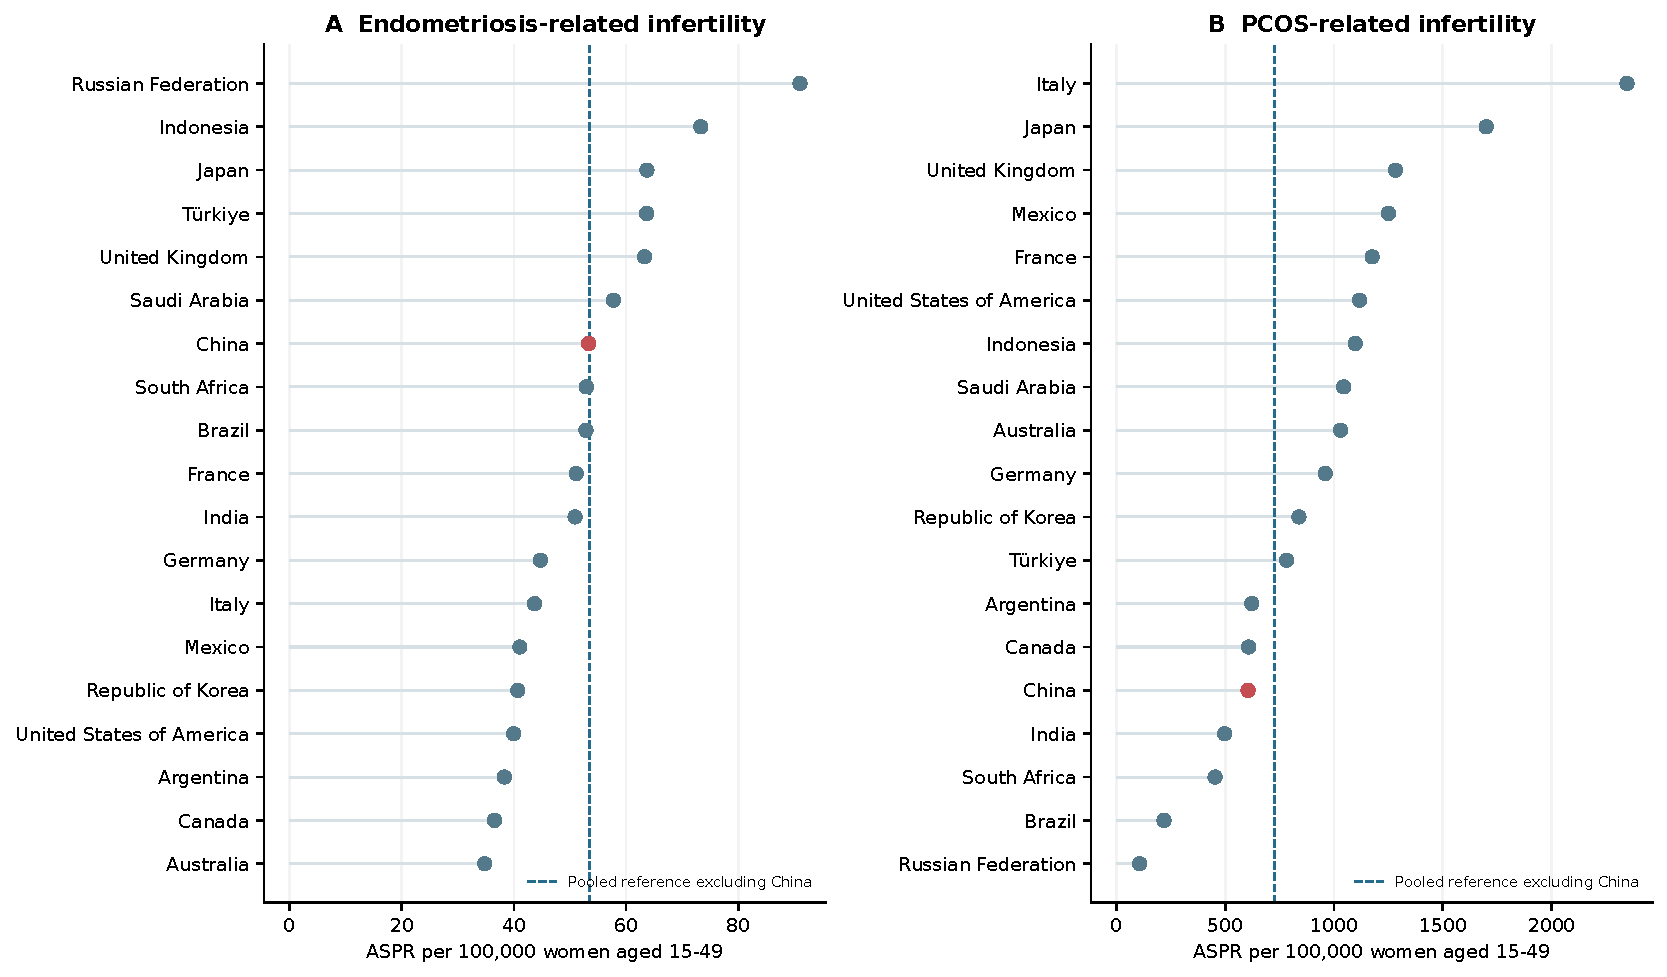
\includegraphics[width=\textwidth]{figures/fig1_country_comparison_2023.pdf}
\caption{Country-specific restricted-age standardized prevalence rates in 2023. Red points denote China; dashed lines show the age-specific population-pooled reference excluding China. Values are point estimates without propagated uncertainty; ranks are descriptive.}\label{fig:countries}\end{figure}
\begin{figure}[p]\centering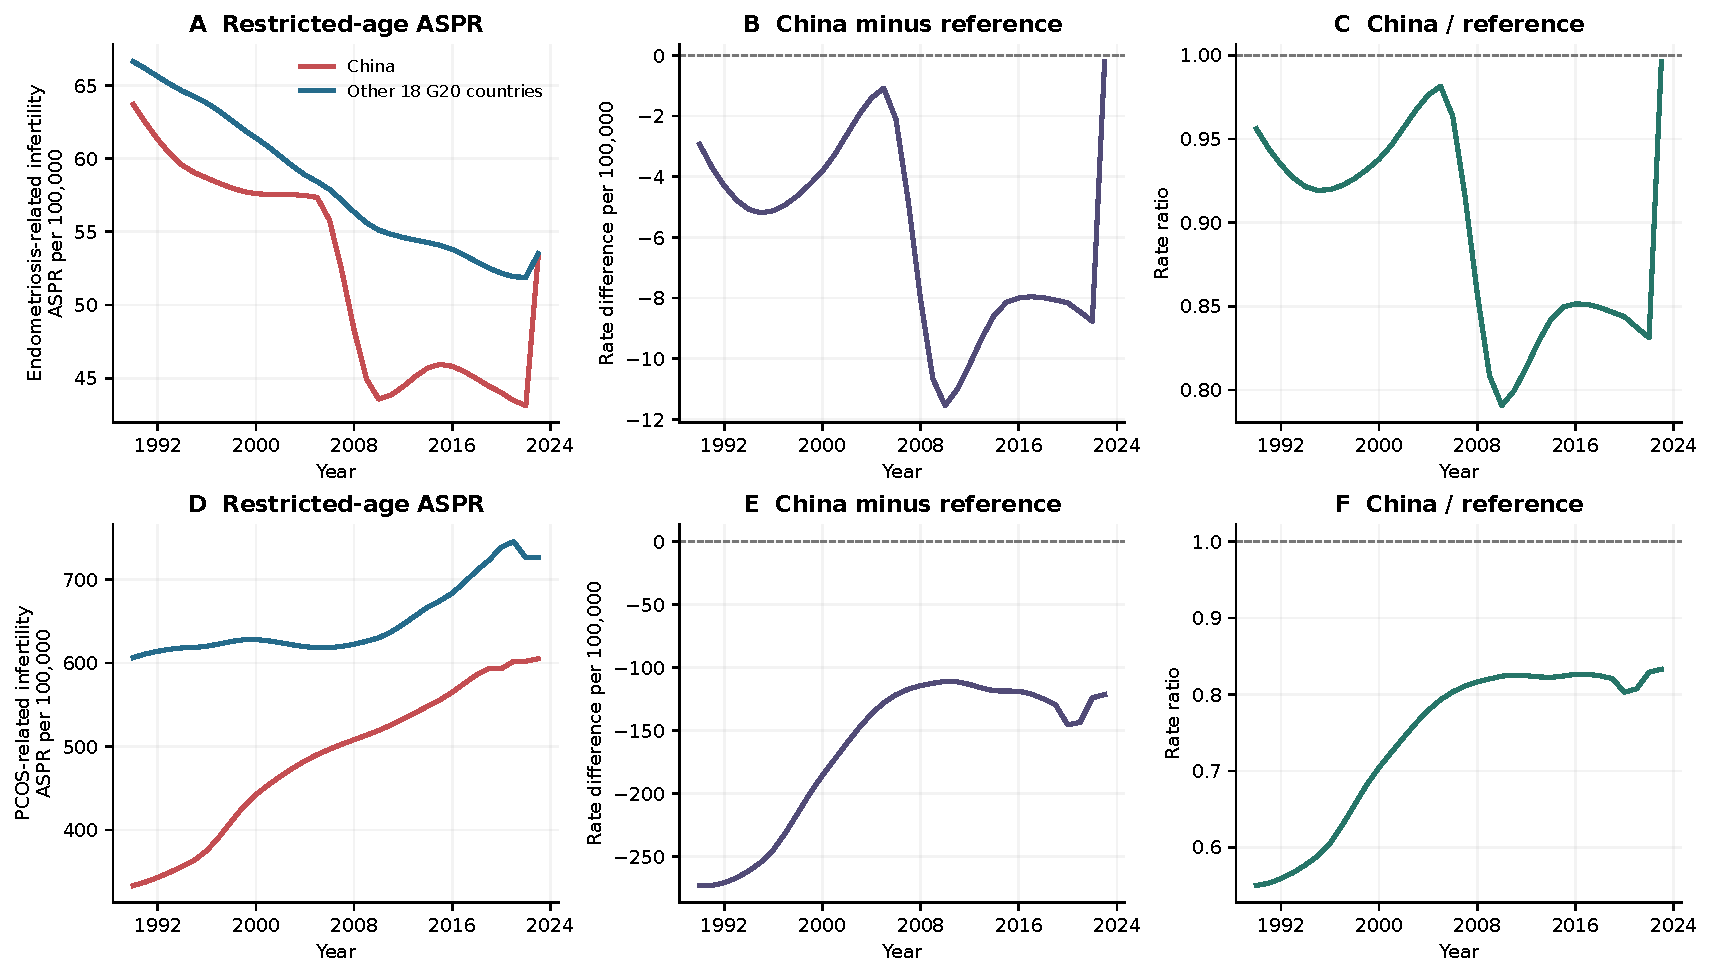
\includegraphics[width=\textwidth]{figures/fig2_trends_and_disparities.pdf}
\caption{Annual standardized prevalence rates, China-minus-reference differences and China/reference ratios. All rates use the same standard weights normalized within ages 15--49. The terminal-year endometriosis change is a feature of the downloaded estimates; it is not interpreted as an independently validated epidemiological shift.}\label{fig:trends}\end{figure}
\begin{figure}[p]\centering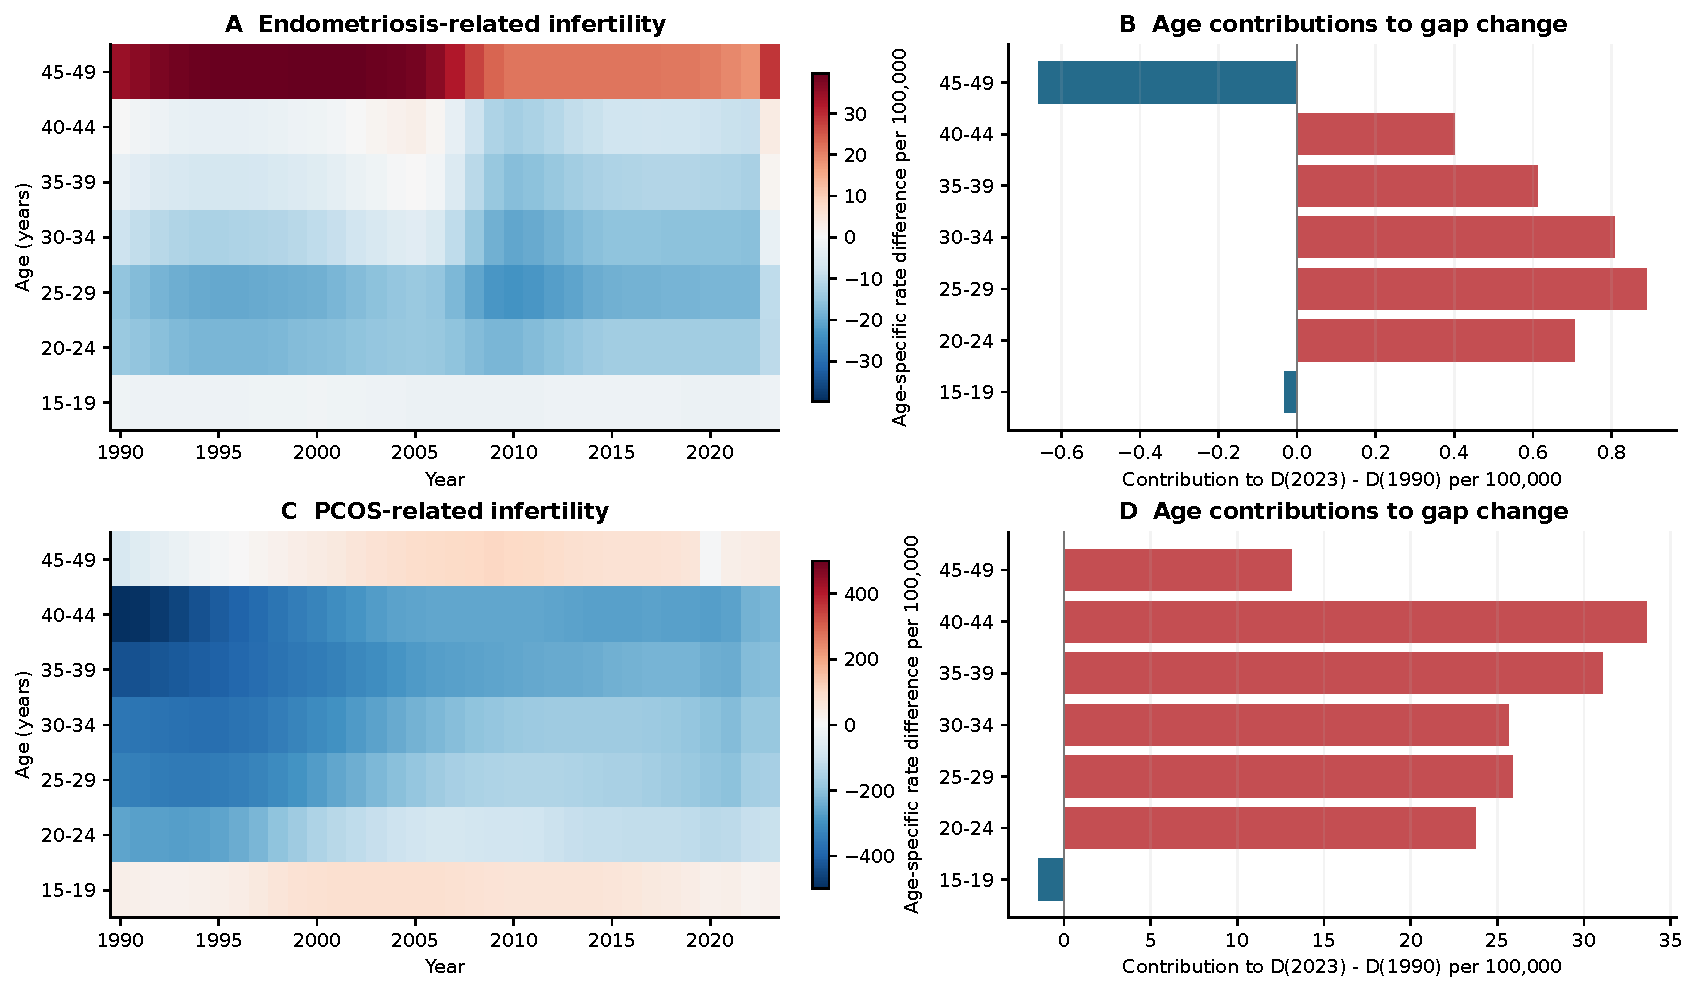
\includegraphics[width=\textwidth]{figures/fig3_age_disparities.pdf}
\caption{Age-specific contrasts and contributions to the change in the standardized prevalence difference, 1990--2023. Heatmaps show unstandardized age-specific China-minus-reference rates. Bars show each age group's standard-weighted contribution to $D_{2023}-D_{1990}$. Positive values indicate movement toward a more positive signed contrast, rather than improvement.}\label{fig:ages}\end{figure}
\begin{figure}[p]\centering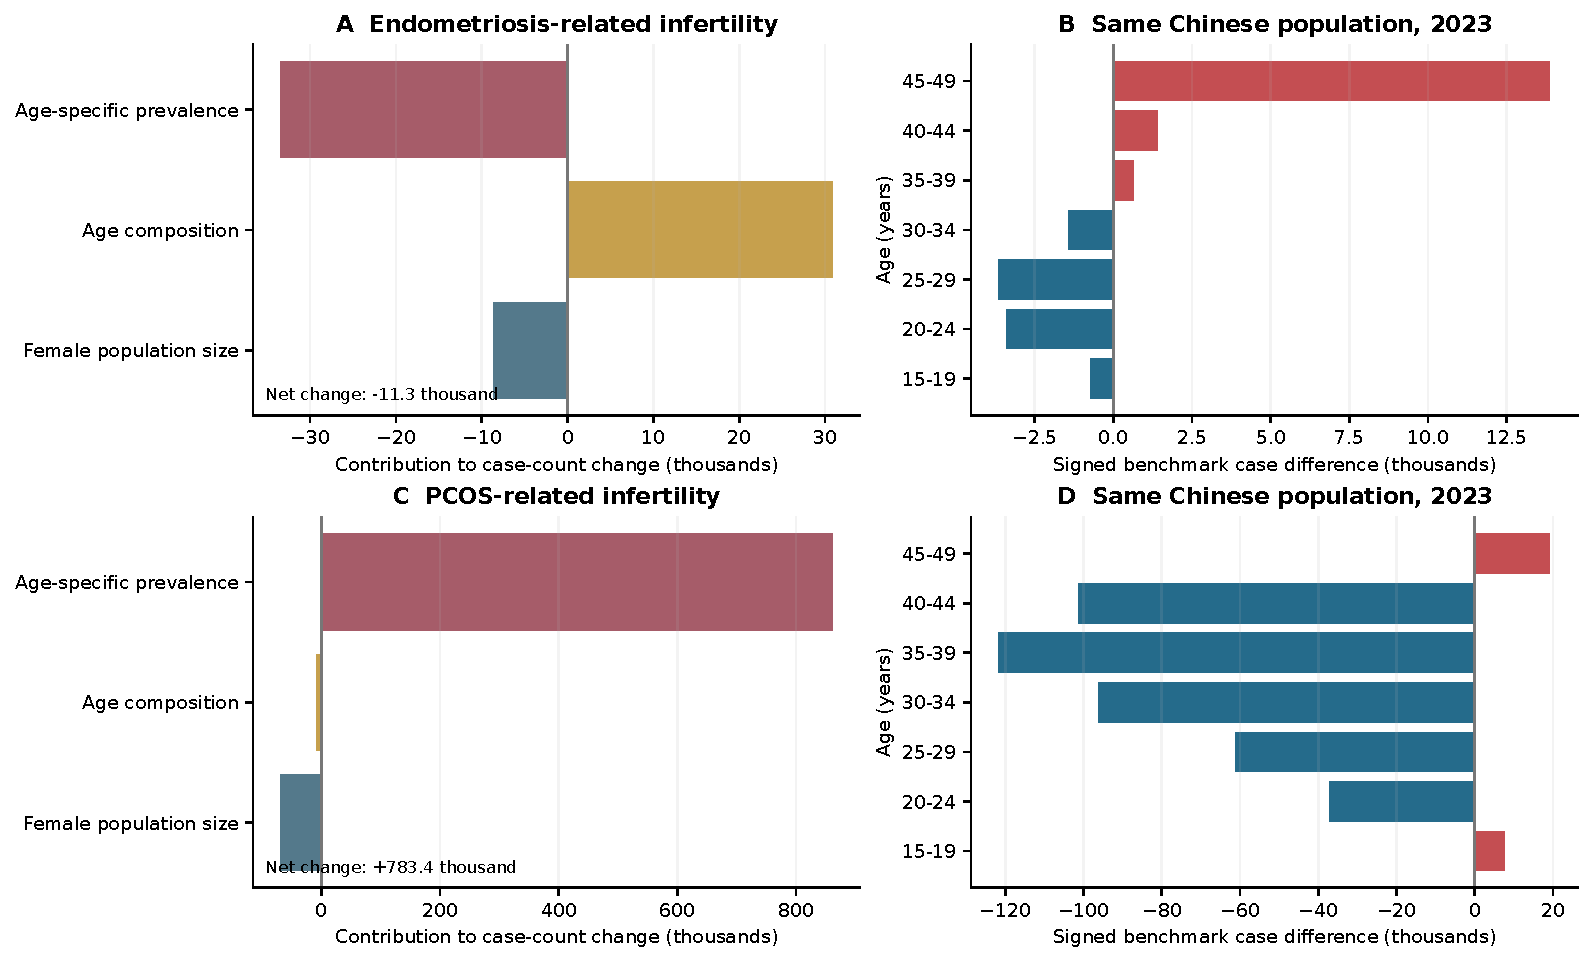
\includegraphics[width=\textwidth]{figures/fig4_decomposition_and_benchmark.pdf}
\caption{China's Shapley decomposition of prevalent case-count changes, 1990--2023, and age-specific same-population benchmark differences in 2023. Decomposition contributions sum to the net change. Benchmarks use China's actual age-specific female populations and are not estimates of preventable cases. The color scheme separates accounting components on the left and contrast signs on the right.}\label{fig:decomp}\end{figure}
\clearpage
\appendix
\section{Supplementary methods and results}
\renewcommand{\thetable}{S\arabic{table}}\setcounter{table}{0}
\renewcommand{\thefigure}{S\arabic{figure}}\setcounter{figure}{0}
\begin{table}[htbp]\centering\small
\caption{Restricted-age standardized YLD rates and YLD totals.}\label{tab:yld}
\setlength{\tabcolsep}{3.5pt}
\begin{tabular}{llrrrrrr}\toprule
 & & \multicolumn{2}{c}{YLDs, thousands} & \multicolumn{2}{c}{Rate per 100,000} & & \\
Cause & Year & China & Reference & China & Reference & $D$ & $RR$\\\midrule
Endometriosis & 1990 & 1.0 & 2.2 & 0.34 & 0.39 & -0.05 & 0.872 \\
Endometriosis & 2023 & 1.0 & 2.6 & 0.29 & 0.31 & -0.02 & 0.934 \\
PCOS & 1990 & 5.9 & 20.5 & 1.80 & 3.59 & -1.79 & 0.502 \\
PCOS & 2023 & 10.1 & 35.5 & 3.31 & 4.22 & -0.91 & 0.784 \\
\bottomrule
\end{tabular}
\caption*{All values are derived point estimates. YLD: years lived with disability.}
\end{table}
\begin{table}[htbp]\centering\small
\caption{Endpoint sensitivity added after inspection of terminal-year estimates.}\label{tab:endpoint}
\begin{tabular}{llrrrrr}\toprule
Cause & End year & China ASPR & Ref. ASPR & $D$ & $RR$ & $D_T-D_{1990}$\\\midrule
Endometriosis & 2021 & 43.48 & 51.93 & -8.45 & 0.837 & -5.52 \\
Endometriosis & 2022 & 43.13 & 51.89 & -8.76 & 0.831 & -5.83 \\
Endometriosis & 2023 & 53.30 & 53.51 & -0.20 & 0.996 & 2.73 \\
PCOS & 2021 & 601.79 & 745.23 & -143.44 & 0.808 & 129.47 \\
PCOS & 2022 & 602.09 & 726.09 & -124.00 & 0.829 & 148.91 \\
PCOS & 2023 & 605.08 & 726.45 & -121.38 & 0.833 & 151.54 \\
\bottomrule
\end{tabular}
\caption*{The source release remains GBD 2023 in all rows. Ending in 2021 is not substitution of GBD 2021 estimates. Rate units: per 100,000 women.}
\end{table}
\begin{table}[htbp]\centering\small
\caption{Conditional trend sensitivity for prevalence, 1990--2023.}\label{tab:trends}
\begin{tabular}{lllrr}\toprule
Location & Cause & Model & AAPC (\%) & Conditional 95\% CI\\\midrule
China & Endometriosis & OLS, 0--2 knots & -0.86 & (-1.00, -0.71) \\
China & Endometriosis & AR(1), fixed knots & -0.82 & (-0.99, -0.65) \\
China & Endometriosis & OLS, 0--3 knots & -0.86 & (-1.00, -0.71) \\
China & PCOS & OLS, 0--2 knots & 1.89 & (1.85, 1.93) \\
China & PCOS & AR(1), fixed knots & 1.94 & (1.81, 2.08) \\
China & PCOS & OLS, 0--3 knots & 1.84 & (1.80, 1.87) \\
Reference & Endometriosis & OLS, 0--2 knots & -0.74 & (-0.78, -0.71) \\
Reference & Endometriosis & AR(1), fixed knots & -0.74 & (-0.78, -0.69) \\
Reference & Endometriosis & OLS, 0--3 knots & -0.72 & (-0.75, -0.68) \\
Reference & PCOS & OLS, 0--2 knots & 0.53 & (0.49, 0.58) \\
Reference & PCOS & AR(1), fixed knots & 0.49 & (0.42, 0.57) \\
Reference & PCOS & OLS, 0--3 knots & 0.57 & (0.53, 0.61) \\
\bottomrule
\end{tabular}
\caption*{Intervals condition on selected knots and fixed GBD point estimates. AR(1) retains the knots selected by OLS with up to two knots. These intervals exclude GBD, knot-selection and structural model uncertainty. Full periods, measures, knots and residual-correlation estimates are in the accompanying CSV.}
\end{table}
\clearpage
\begin{table}[htbp]\centering\small
\caption{Age-specific forecast-validation MAE ratios relative to the naive baseline.}\label{tab:forecast}
\begin{tabular}{llccc}\toprule
Cause & Model & Rolling: min--max & Last 10 years: min--max & Retained\\\midrule
Endometriosis & ARIMA & 0.87--1.30 & 0.93--1.80 & No \\
Endometriosis & ETS & 1.00--1.51 & 0.86--2.10 & No \\
PCOS & ARIMA & 0.19--2.20 & 0.06--1.38 & No \\
PCOS & ETS & 0.20--1.79 & 0.09--1.28 & No \\
\bottomrule
\end{tabular}
\caption*{Ranges span seven age groups. Values below 1 favor the candidate. Retention required every age-specific ratio to be below 0.9 in both schemes, with complete predictions. The rule was specified before running this exploratory module, not externally preregistered. Rolling MAE combines horizons 1, 3 and 5; the holdout combines horizons 1--10.}
\end{table}
\begin{table}[htbp]\centering\small
\caption{Primary and secondary infertility prevalence contrasts at the endpoints.}\label{tab:strata}
\setlength{\tabcolsep}{4pt}
\begin{tabular}{lllrrrr}\toprule
Cause & Type & Year & China ASPR & Ref. ASPR & $D$ & $RR$\\\midrule
Endometriosis & Primary & 1990 & 4.92 & 19.64 & -14.72 & 0.250 \\
Endometriosis & Primary & 2023 & 4.94 & 12.87 & -7.94 & 0.384 \\
Endometriosis & Secondary & 1990 & 58.78 & 46.98 & 11.79 & 1.251 \\
Endometriosis & Secondary & 2023 & 48.37 & 40.63 & 7.73 & 1.190 \\
PCOS & Primary & 1990 & 44.70 & 214.64 & -169.94 & 0.208 \\
PCOS & Primary & 2023 & 97.35 & 220.89 & -123.54 & 0.441 \\
PCOS & Secondary & 1990 & 288.86 & 391.84 & -102.98 & 0.737 \\
PCOS & Secondary & 2023 & 507.72 & 505.56 & 2.16 & 1.004 \\
\bottomrule
\end{tabular}
\caption*{Rates per 100,000 women, standardized within ages 15--49. All quantities are point estimates. Annual rates use original Number divided by matching GBD 2023 population; original endpoint Rate independently reproduced these results. Primary and secondary estimates sum to the total point estimates.}
\end{table}
\subsection{Acquisition and computation audit}
The official query identifiers were:
\begin{description}
\item[Burden:] \texttt{1b13e3376135ab41a4bc5e0ffc60e84f}.
\item[Population:] \texttt{916826fb285f8d3c3e53117dd2133406}.
\item[Pilot:] \texttt{0daed0e53f5ad8ebdf0dc00c23ccd110}.
\item[Annual strata:] \texttt{416daf735b9fc79bec35506514424e73}.
\item[Endpoint strata:] \texttt{76c5523c52f32caf342843daf2326fa4}.
\end{description}
Raw uncertainty limits remain in the original CSVs. Country and outcome mappings, source hashes, rounding sensitivities and all analytical tables are separate machine-readable files. Nine automated checks cover core accounting identities, the complete data grid, denominator consistency and outcome gates; temporary artificial test fixtures were not used as research data.

The protocol was written before analysis but was not externally preregistered. The endpoint and weight-rounding sensitivities were added following quality inspection. Forecasting remained exploratory and was withheld after failed comparative validation. Primary/secondary stratification was completed using annual Number exports and independent endpoint Number/Rate checks. External survey comparisons and future population scenarios were not completed; they were optional extensions. The annual stratum rate reconstruction reduced redundant metrics within the remaining GBD download allowance.

\subsection{GATHER reporting map}
This map applies GATHER to the secondary analysis; upstream input reconstruction and primary disease estimation belong to the original GBD study. It is not a claim of independent GBD model replication.
\small
\begin{longtable}{>{\raggedright\arraybackslash}p{0.08\textwidth}>{\raggedright\arraybackslash}p{0.27\textwidth}>{\raggedright\arraybackslash}p{0.54\textwidth}}
\toprule Item & Topic & Location or applicability\\\midrule\endhead
1 & Indicators and populations & Methods: causes, ages, female sex, fixed countries and 1990--2023.\\
2 & Funding & Declarations: author-supplied information remains pending.\\
3 & Data identification and access & Official Results Tool, download date, query identifiers and cited GBD methods.\\
4 & Eligibility and exclusions & Exact outcome filters and completeness gates; no country removals from the main set. Sensitivity exclusions are explicit.\\
5 & Source characteristics & GBD model outputs, dimensional mappings and acquisition audit. Original source-study characteristics are documented by GBD.\\
6 & Potential input biases & Discussion: sparse evidence, diagnostic heterogeneity, attribution and modeled denominators.\\
7 & Other inputs & Matching GBD population and published standard weights with provenance.\\
8 & Input data access & CSVs retained in the research archive; source institution IHME and exact queries identified for reproducibility.\\
9 & Conceptual overview & Equations for within-age pooling, standardization, contrasts and decomposition.\\
10 & Analytical detail & Normalization, validation, comparison, decomposition, trend and sensitivity methods and scripts.\\
11 & Candidate evaluation and selection & Segmented-model BIC, training AICc and explicit forecast-retention criterion.\\
12 & Evaluation results & Reference, endpoint, AR(1), rounding and forecast-validation results.\\
13 & Uncertainty methods and scope & Joint draws unavailable; no propagated derived intervals; conditional trend interval scope stated.\\
14 & Source code access & GitHub repository, pinned dependencies and executable scripts.\\
15 & Machine-readable estimates & Complete derived CSV tables accompany the paper.\\
16 & Quantitative uncertainty & Incomplete for derived estimates: marginal source limits retained but cannot substitute for joint uncertainty. Trend intervals are conditional only.\\
17 & Interpretation and prior evidence & Discussion compares prior GBD studies. Release-to-release differences were not estimated.\\
18 & Limitations & Discussion: endpoint, reference, denominator, source, rounding and inference limitations.\\\bottomrule
\end{longtable}
\normalsize
\clearpage
\begin{figure}[p]\centering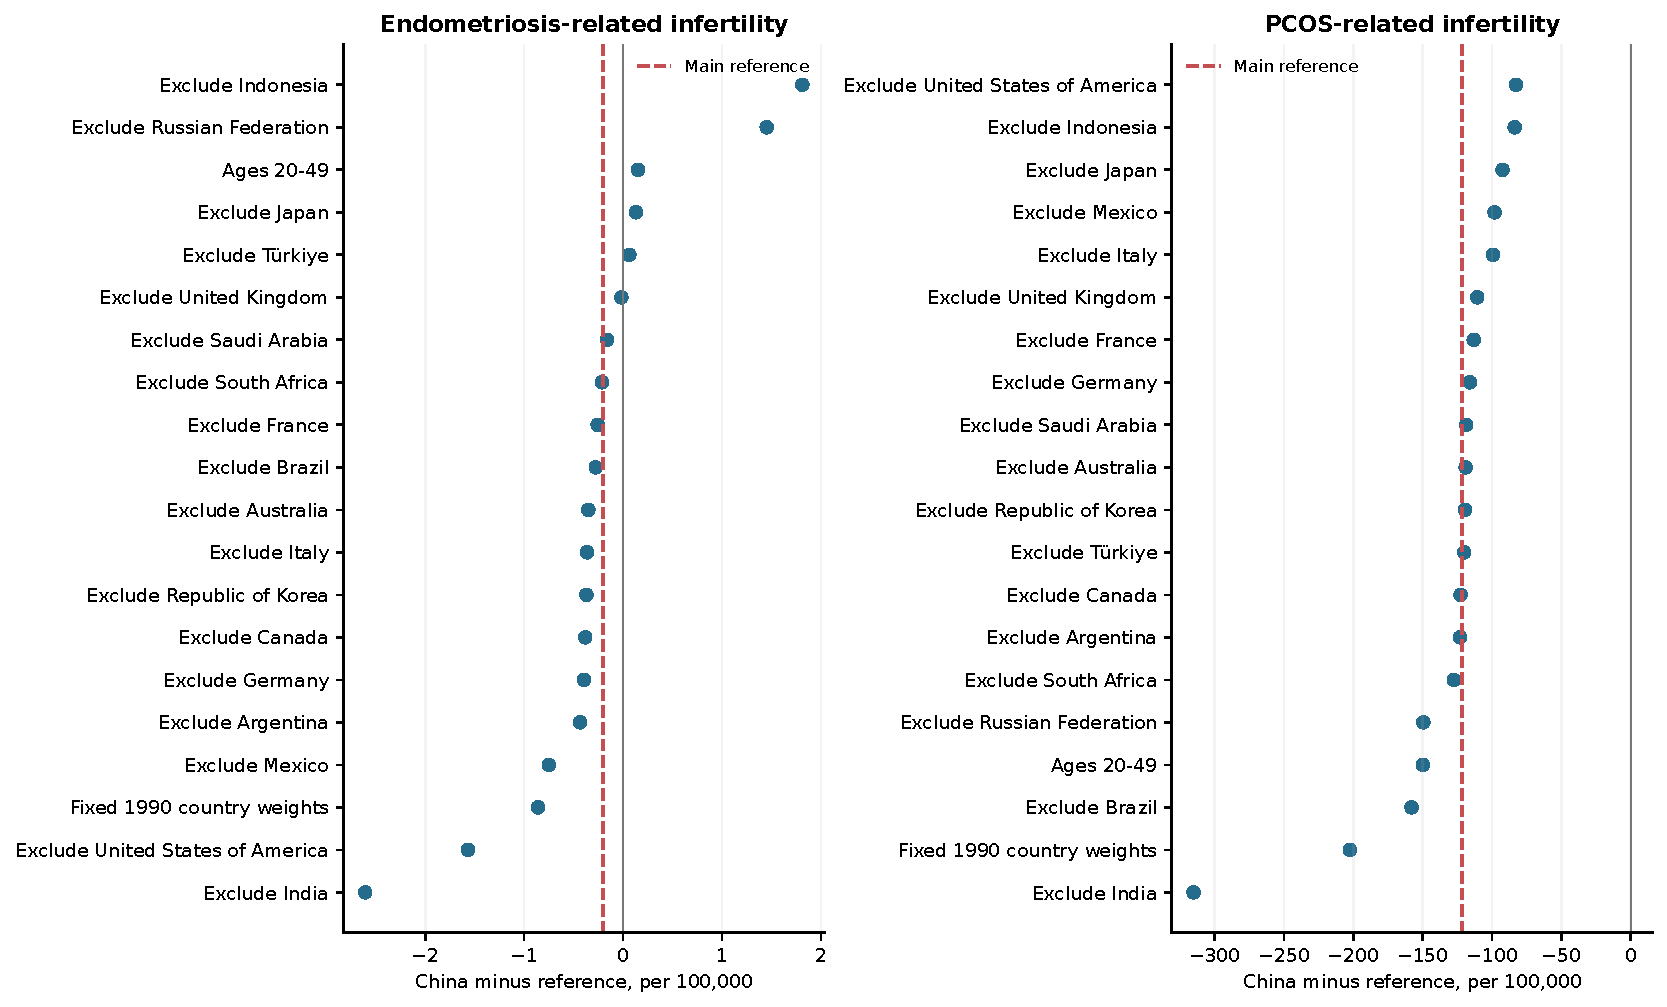
\includegraphics[width=\textwidth]{figures/figS1_reference_sensitivity.pdf}
\caption{Sensitivity of the 2023 prevalence difference to reference-country exclusions, fixed 1990 country shares within ages, and restriction to ages 20--49. Dashed lines show the main 15--49 comparison. PCOS signs are stable; endometriosis signs vary. All are point estimates.}\label{fig:sensitivity}\end{figure}
\begin{figure}[p]\centering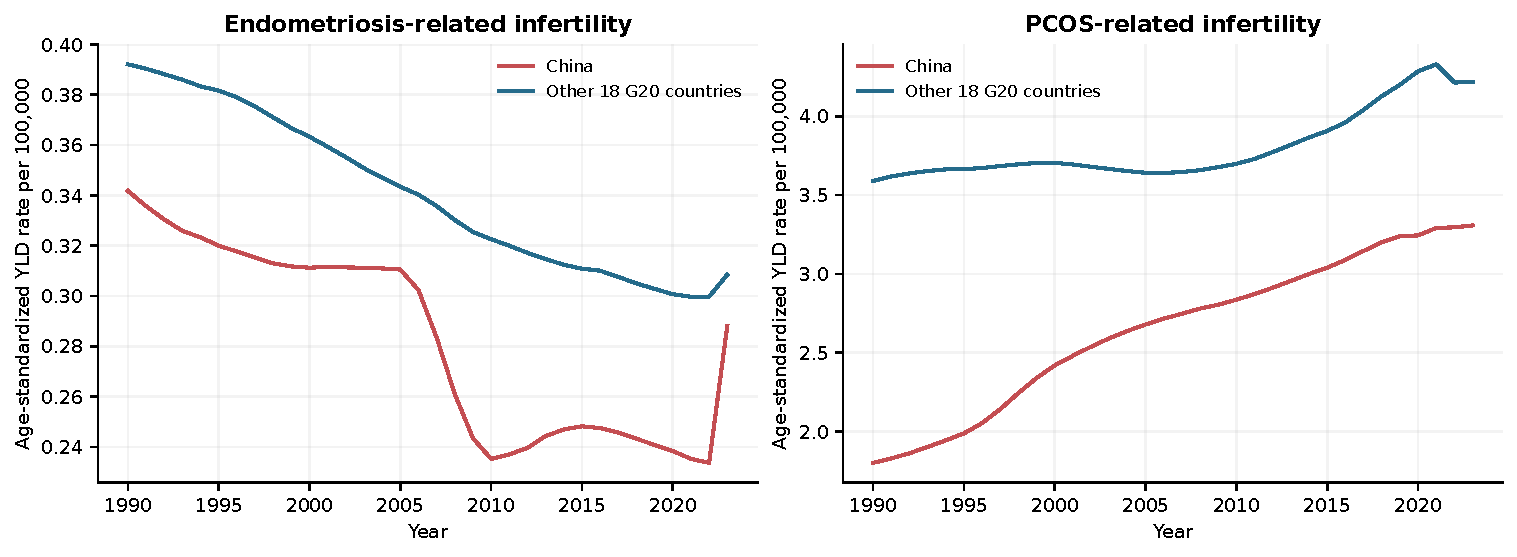
\includegraphics[width=\textwidth]{figures/figS2_yld_trends.pdf}
\caption{Restricted-age standardized YLD rates for both infertility causes, 1990--2023. These are infertility-impairment YLD rates rather than the total disability burden of either underlying disease.}\label{fig:yld}\end{figure}
\begin{figure}[p]\centering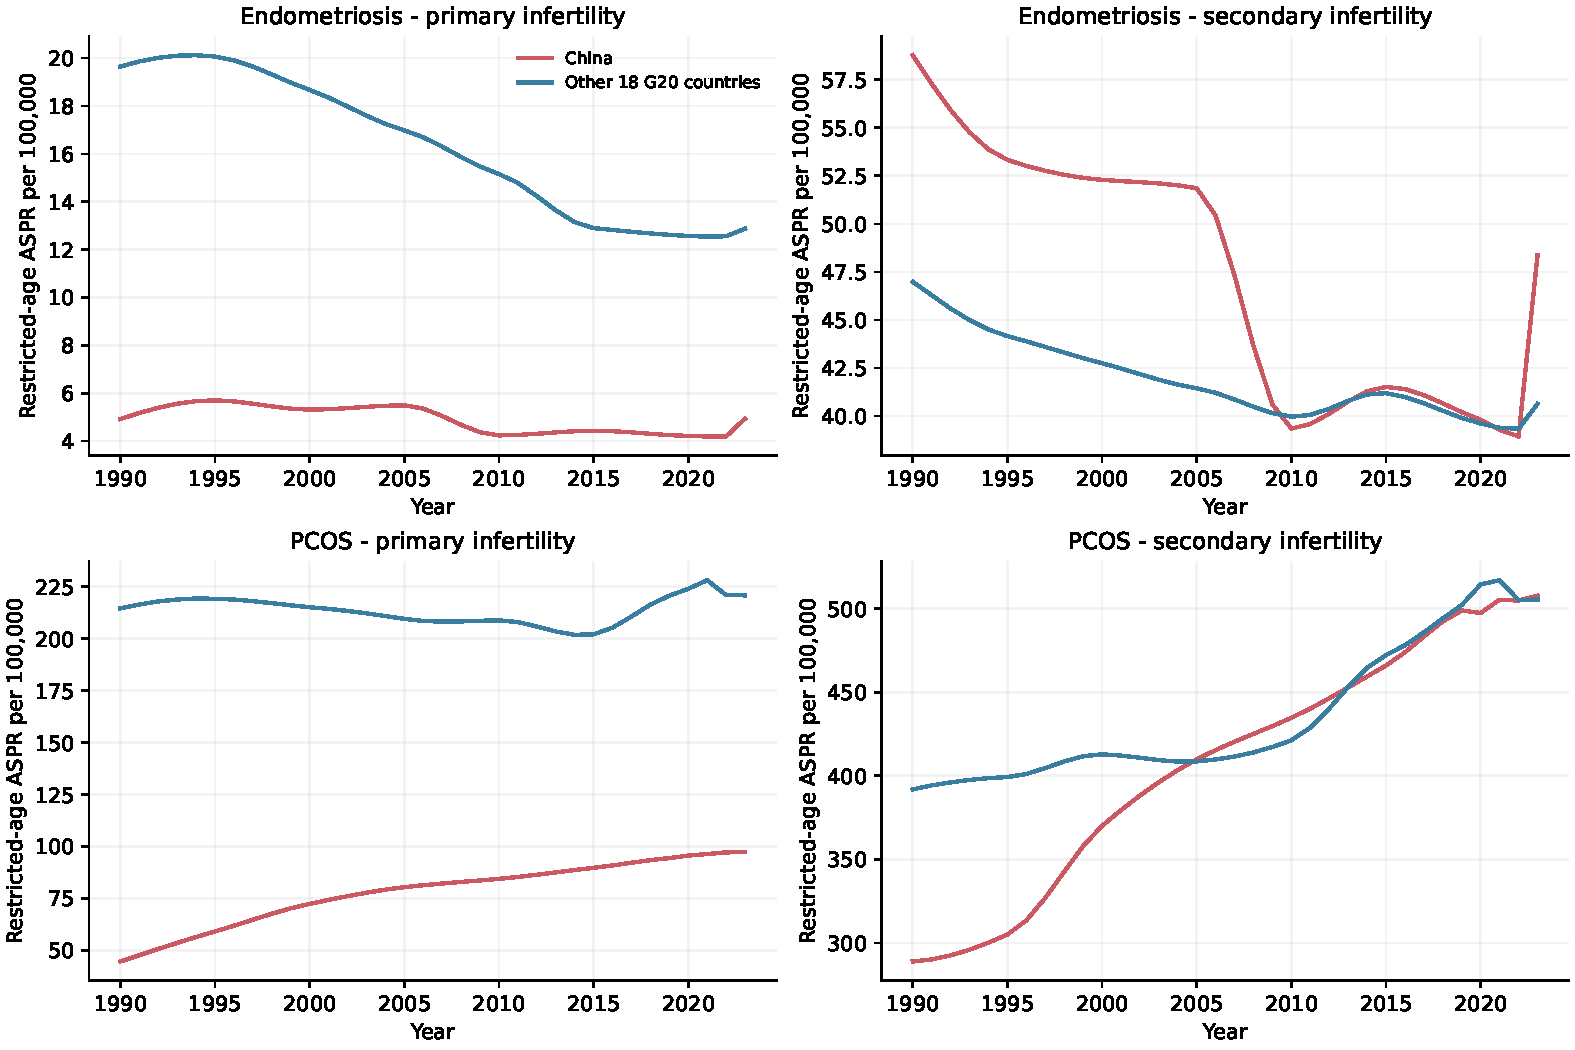
\includegraphics[width=\textwidth]{figures/figS3_infertility_strata.pdf}
\caption{Restricted-age standardized prevalence by primary and secondary infertility, 1990--2023. China and the reference have contrasting primary-infertility rates, while secondary-infertility comparisons vary over time. The 2023 secondary endometriosis change contributes to the terminal-year total contrast. These are modeled point trajectories without propagated uncertainty.}\label{fig:strata}\end{figure}
\end{document}
